\documentclass[11pt,oneside]{article}
\usepackage[T1]{fontenc}
\usepackage[utf8]{inputenc}
% \usepackage{lmodern}
%\usepackage[adobe-utopia,uppercase=upright,greeklowercase=upright]{mathdesign}
\usepackage[adobe-utopia]{mathdesign}
%\usepackage{minionpro}
% \usepackage{pifont}
% \usepackage{amssymb}
\usepackage{amsmath}
\usepackage[francais]{babel}
% \usepackage[francais]{varioref}
\usepackage[dvips]{graphicx}

\usepackage{framed}
\usepackage[normalem]{ulem}
\usepackage{fancyhdr}
\usepackage{titlesec}
\usepackage{vmargin}
\usepackage{longtable}

\usepackage{ifthen}


%\usepackage{epsfig}
\usepackage{subfig}

\usepackage{multirow}
\usepackage{multicol} % Portions de texte en colonnes
\usepackage{flafter}%floatants après la référence



\usepackage{color}
\usepackage{colortbl}


\definecolor{gris25}{gray}{0.75}
\definecolor{bleu}{RGB}{18,33,98}
\definecolor{bleuf}{RGB}{42,94,171}
\definecolor{bleuc}{RGB}{231,239,247}
\definecolor{rougef}{RGB}{185,18,27}
\definecolor{rougec}{RGB}{255,230,231}
\definecolor{vertf}{RGB}{103,126,82}
\definecolor{vertc}{RGB}{220,255,191}

\newenvironment{rem}[1][\hsize]%
{%
    \def\FrameCommand
    {%
\rotatebox{90}{\textit{\textsf{Remarque}}} 
        {\color{bleuf}\vrule width 3pt}%
        \hspace{0pt}%must no space.
        \fboxsep=\FrameSep\colorbox{bleuc}%
    }%
    \MakeFramed{\hsize#1\advance\hsize-\width\FrameRestore}%
}%
{\endMakeFramed}%


\newenvironment{savoir}[1][\hsize]%
{%
    \def\FrameCommand
    {%
\rotatebox{90}{\textit{\textsf{Savoir}}} 
        {\color{bleuf}\vrule width 3pt}%
        \hspace{0pt}%must no space.
        \fboxsep=\FrameSep\colorbox{bleuc}%
    }%
    \MakeFramed{\hsize#1\advance\hsize-\width\FrameRestore}%
}%
{\endMakeFramed}%

\newenvironment{prob}[1][\hsize]%
{%
    \def\FrameCommand%
    {%
\rotatebox{90}{\textit{\textsf{ Problématique}}} 
        {\color{rougef}\vrule width 3pt}%
        \hspace{0pt}%must no space.
        \fboxsep=\FrameSep\colorbox{rougec}%
    }%
    \MakeFramed{\hsize#1\advance\hsize-\width\FrameRestore}%
}%
{\endMakeFramed}%

\newenvironment{obj}[1][\hsize]%
{%
    \def\FrameCommand%
    {%
\rotatebox{90}{\textit{\textsf{ $\;$}}} 
        {\color{rougef}\vrule width 3pt}%
        \hspace{0pt}%must no space.
        \fboxsep=\FrameSep\colorbox{rougec}%
    }%
    \MakeFramed{\hsize#1\advance\hsize-\width\FrameRestore}%
}%
{\endMakeFramed}%

\newenvironment{defi}[1][\hsize]%
{%
    \def\FrameCommand%
    {%
\rotatebox{90}{\textit{\textsf{Définition\\}}} 
        {\color{bleuf}\vrule width 3pt}%
        \hspace{0pt}%must no space.
        \fboxsep=\FrameSep\colorbox{bleuc}%
    }%
    \MakeFramed{\hsize#1\advance\hsize-\width\FrameRestore}%
}%
{\endMakeFramed}%


\newenvironment{hypo}[1][\hsize]%
{%
    \def\FrameCommand%
    {%
\rotatebox{90}{\textit{\textsf{Hypothèse\\}}} 
        {\color{bleuf}\vrule width 3pt}%
        \hspace{0pt}%must no space.
        \fboxsep=\FrameSep\colorbox{bleuc}%
    }%
    \MakeFramed{\hsize#1\advance\hsize-\width\FrameRestore}%
}%
{\endMakeFramed}%


\newenvironment{prop}[1][\hsize]%
{%
    \def\FrameCommand%
    {%
\rotatebox{90}{\textit{\textsf{Propriété\\}}} 
        {\color{bleuf}\vrule width 3pt}%
        \hspace{0pt}%must no space.
        \fboxsep=\FrameSep\colorbox{bleuc}%
    }%
    \MakeFramed{\hsize#1\advance\hsize-\width\FrameRestore}%
}%
{\endMakeFramed}%

\newenvironment{props}[1][\hsize]%
{%
    \def\FrameCommand%
    {%
\rotatebox{90}{\textit{\textsf{Propriétés\\}}} 
        {\color{bleuf}\vrule width 3pt}%
        \hspace{0pt}%must no space.
        \fboxsep=\FrameSep\colorbox{bleuc}%
    }%
    \MakeFramed{\hsize#1\advance\hsize-\width\FrameRestore}%
}%
{\endMakeFramed}%

\newenvironment{exemple}[1][\hsize]%
{%
    \def\FrameCommand%
    {%
\rotatebox{90}{\textit{\textsf{Exemple\\}}} 
        {\color{vertf}\vrule width 3pt}%
        \hspace{0pt}%must no space.
        \fboxsep=\FrameSep\colorbox{vertc}%
    }%
    \MakeFramed{\hsize#1\advance\hsize-\width\FrameRestore}%
}%
{\endMakeFramed}%

\newenvironment{resultat}[1][\hsize]%
{%
    \def\FrameCommand%
    {%
\rotatebox{90}{\textit{\textsf{Résultat\\}}} 
        {\color{rougef}\vrule width 3pt}%
        \hspace{0pt}%must no space.
        \fboxsep=\FrameSep\colorbox{rougec}%
    }%
    \MakeFramed{\hsize#1\advance\hsize-\width\FrameRestore}%
}%
{\endMakeFramed}%

\newenvironment{methode}[1][\hsize]%
{%
    \def\FrameCommand%
    {%
\rotatebox{90}{\textit{\textsf{Méthode\\}}} 
        {\color{rougef}\vrule width 3pt}%
        \hspace{0pt}%must no space.
        \fboxsep=\FrameSep\colorbox{rougec}%
    }%
    \MakeFramed{\hsize#1\advance\hsize-\width\FrameRestore}%
}%
{\endMakeFramed}%

\newenvironment{theo}[1][\hsize]%
{%
    \def\FrameCommand%
    {%
\rotatebox{90}{\textit{\textsf{Théorème\\}}} 
        {\color{rougef}\vrule width 3pt}%
        \hspace{0pt}%must no space.
        \fboxsep=\FrameSep\colorbox{rougec}%
    }%
    \MakeFramed{\hsize#1\advance\hsize-\width\FrameRestore}%
}%
{\endMakeFramed}%

\newenvironment{warn}[1][\hsize]%
{%
    \def\FrameCommand%
    {%
\rotatebox{90}{\textit{\textsf{Attention\\}}} 
        {\color{rougef}\vrule width 3pt}%
        \hspace{0pt}%must no space.
        \fboxsep=\FrameSep\colorbox{rougec}%
    }%
    \MakeFramed{\hsize#1\advance\hsize-\width\FrameRestore}%
}%
{\endMakeFramed}%

% \usepackage{pstricks}
%\usepackage{minitoc}
% \setcounter{minitocdepth}{4}

\setcounter{tocdepth}{2}

% \mtcselectlanguage{french} 

%\usepackage{draftcopy}% "Brouillon"
% \usepackage{floatflt}
\usepackage{psfrag}
%\usepackage{listings} % Permet d'insérer du code de programmation
\renewcommand{\baselinestretch}{1.2}

% Changer la numérotation des figures :
% ------------------------------------
% \makeatletter
% \renewcommand{\thefigure}{\ifnum \c@section>\z@ \thesection.\fi
%  \@arabic\c@figure}
% \@addtoreset{figure}{section}
% \makeatother
 


%%%%%%%%%%%%
% Définition des vecteurs %
%%%%%%%%%%%%
 \newcommand{\vect}[1]{\overrightarrow{#1}}

%%%%%%%%%%%%
% Définition des torseusr %
%%%%%%%%%%%%

 \newcommand{\torseur}[1]{%
\left\{{#1}\right\}
}

\newcommand{\torseurcin}[3]{%
\left\{\mathcal{#1} \left(#2/#3 \right) \right\}
}

\newcommand{\torseurstat}[3]{%
\left\{\mathcal{#1} \left(#2\rightarrow #3 \right) \right\}
}

 \newcommand{\torseurc}[8]{%
%\left\{#1 \right\}=
\left\{
{#1}
\right\}
 = 
\left\{%
\begin{array}{cc}%
{#2} & {#5}\\%
{#3} & {#6}\\%
{#4} & {#7}\\%
\end{array}%
\right\}_{#8}%
}

 \newcommand{\torseurcol}[7]{
\left\{%
\begin{array}{cc}%
{#1} & {#4}\\%
{#2} & {#5}\\%
{#3} & {#6}\\%
\end{array}%
\right\}_{#7}%
}

 \newcommand{\torseurl}[3]{%
%\left\{\mathcal{#1}\right\}_{#2}=%
\left\{%
\begin{array}{l}%
{#1} \\%
{#2} %
\end{array}%
\right\}_{#3}%
}

 \newcommand{\vectv}[3]{%
\vect{V\left( {#1} \in {#2}/{#3}\right)}
}


\newcommand{\vectf}[2]{%
\vect{R\left( {#1} \rightarrow {#2}\right)}
}

\newcommand{\vectm}[3]{%
\vect{\mathcal{M}\left( {#1}, {#2} \rightarrow {#3}\right)}
}


 \newcommand{\vectg}[3]{%
\vect{\Gamma \left( {#1} \in {#2}/{#3}\right)}
}

 \newcommand{\vecto}[2]{%
\vect{\Omega\left( {#1}/{#2}\right)}
}
% }$$\left\{\mathcal{#1} \right\}_{#2} =%
% \left\{%
% \begin{array}{c}%
%  #3 \\%
%  #4 %
% \end{array}%
% \right\}_{#5}}

%  ------------------------------------------
% | Modification du formatage des sections : | 
%  ------------------------------------------

% Grands titres :
% ---------------

\newcommand{\titre}[1]{%
\begin{center}
      \bigskip
      \rule{\textwidth}{1pt}
      \par\vspace{0.1cm}
      
      \textbf{\large #1}
      \par\rule{\textwidth}{1pt}
    \end{center}
    \bigskip
  }

% Supprime le numéro du chapitre dans la numérotation des sections:
% -----------------------------------------------------------------
\makeatletter
\renewcommand{\thesection}{\@arabic\c@section}
\makeatother


% \titleformat{\chapter}[display]
% {\normalfont\Large\filcenter}
% {}
% {1pc}
% {\titlerule[1pt]
%   \vspace{1pc}%
%   \Huge}[\vspace{1ex}%
% \titlerule]


%%%% Chapitres Comme PY Pechard %%%%%%%%%
% numéro du chapitre
\DeclareFixedFont{\chapnumfont}{OT1}{phv}{b}{n}{80pt}
% pour le mot « Chapitre »
\DeclareFixedFont{\chapchapfont}{OT1}{phv}{m}{it}{40pt}
% pour le titre
\DeclareFixedFont{\chaptitfont}{T1}{phv}{b}{n}{25pt}

\definecolor{gris}{gray}{0.75}
\titleformat{\chapter}[display]%
	{\sffamily}%
	{\filleft\chapchapfont\color{gris}\chaptertitlename\
	\\
	\vspace{12pt}
	\chapnumfont\thechapter}%
	{16pt}%
	{\filleft\chaptitfont}%
	[\vspace{6pt}\titlerule\titlerule\titlerule]

%%%%  Fin Chapitres Comme PY Pechard %%%%%%%%%


% Section, subsection, subsubsection sans serifs :
% % ----------------------------------------------

% \makeatletter
% \renewcommand{\section}{\@startsection{section}{0}{0mm}%
% {\baselineskip}{.3\baselineskip}%
% {\normalfont\sffamily\Large\textbf}}%
% \makeatother

\makeatletter
\renewcommand{\@seccntformat}[1]{{\textcolor{bleu}{\csname
the#1\endcsname}\hspace{0.5em}}}
\makeatother

\makeatletter
\renewcommand{\section}{\@startsection{section}{1}{\z@}%
                       {-4ex \@plus -1ex \@minus -.4ex}%
                       {1ex \@plus.2ex }%
                       {\normalfont\Large\sffamily\bfseries}}%
\makeatother
 
\makeatletter
\renewcommand{\subsection}{\@startsection {subsection}{2}{\z@}
                          {-3ex \@plus -0.1ex \@minus -.4ex}%
                          {0.5ex \@plus.2ex }%
                          {\normalfont\large\sffamily\bfseries}}
\makeatother
 
\makeatletter
\renewcommand{\subsubsection}{\@startsection {subsubsection}{3}{\z@}
                          {-2ex \@plus -0.1ex \@minus -.2ex}%
                          {0.2ex \@plus.2ex }%
                          {\normalfont\large\sffamily\bfseries}}
\makeatother
 
\makeatletter             
\renewcommand{\paragraph}{\@startsection{paragraph}{4}{\z@}%
                                    {-2ex \@plus-.2ex \@minus .2ex}%
                                    {0.1ex}%               
{\normalfont\sffamily\bfseries}}
\makeatother
 
\makeatletter
\renewcommand{\subparagraph}{\@startsection{subparagraph}{5}{\z@}%
                                       {-2ex \@plus-.1ex \@minus .2ex}%
                                       {0.1ex}%
				    {\normalfont\normalsize\sffamily\bfseries}}
\makeatletter
% \makeatletter
% \renewcommand{\subsection}{\@startsection{subsection}{1}{2mm}%
% {\baselineskip}{.3\baselineskip}%
% {\normalfont\sffamily\large\textbf}}%
% \makeatother
% 
% \makeatletter
% \renewcommand{\subsubsection}{\@startsection{subsubsection}{2}{4mm}%
% {\baselineskip}{.15\baselineskip}%
% {\normalfont\sffamily\large\textbf}}%
% \makeatother
% 
% \makeatletter
% \renewcommand{\paragraph}{\@startsection{paragraph}{3}{6mm}%
% {\baselineskip}{.15\baselineskip}%
% {\normalfont\sffamily\large\textbf}}%
% \makeatother
 
\setcounter{secnumdepth}{4}


%  --------
% | Marges |
%  --------


% \setmarginsrb{2.5cm}{1.5cm}{2.5cm}{2cm}{1cm}{1cm}{1cm}{1cm}
\setmarginsrb{1.5cm}{1cm}{1cm}{1.5cm}{1cm}{1cm}{1cm}{1cm}

% Changer les marges localement :
% -----------------------------
\newenvironment{changemargin}[2]{\begin{list}{}{%
\setlength{\topsep}{0pt}%
\setlength{\leftmargin}{0pt}%
\setlength{\rightmargin}{0pt}%
\setlength{\listparindent}{\parindent}%
\setlength{\itemindent}{\parindent}%
\setlength{\parsep}{0pt plus 1pt}%
\addtolength{\leftmargin}{#1}%
\addtolength{\rightmargin}{#2}%
}\item }{\end{list}}



\usepackage{pst-solides3d}
\usepackage{titletoc}
\titlecontents{chapter}[+3pc]
  {\addvspace{10pt}\sffamily\bfseries}
{\contentslabel[{\pscirclebox[fillstyle=solid,fillcolor=gray!25,
linecolor=gray!25,framesep=4pt]{\textcolor{white}{\thecontentslabel}}}]{2.5pc}}
  {}
  {\dotfill \normalfont\thecontentspage\ }

\titlecontents{section}[3pc]
  {\addvspace{2pt}\sffamily}
  {\contentslabel[\thecontentslabel]{1.8pc}}
  {}
  {\dotfill \normalfont\thecontentspage\ }

\titlecontents{subsection}[5pc]
  {\addvspace{2pt}\sffamily}
  {\contentslabel[\thecontentslabel]{1.8pc}}
  {}
  {\dotfill \normalfont\thecontentspage\ }

\titlecontents{subsubsection}[8pc]
  {\addvspace{2pt}\sffamily}
  {\contentslabel[\thecontentslabel]{3pc}}
  {}
  {\dotfill \normalfont\thecontentspage\ }
%{\;\titlerule\;\normalfont\thecontentspage\ }

\titlecontents{paragraph}[9pc]
  {\addvspace{2pt}\sffamily}
  {\contentslabel[\thecontentslabel]{3.5pc}}
  {}
  {\dotfill \normalfont\thecontentspage\ }




\usepackage[%
    pdftitle={Cinématique - Transmissions mécaniques},
    pdfauthor={Xavier Pessoles},
    colorlinks=true,
    linkcolor=blue,
    citecolor=magenta]{hyperref}
\usepackage{schemabloc}



% \makeatletter \let\ps@plain\ps@empty \makeatother
%% DEBUT DU DOCUMENT
%% =================
\sloppy
\hyphenpenalty 10000

\newcommand{\Pointilles}[1][3]{%
\multido{}{#1}{\makebox[\linewidth]{\dotfill}\\[\parskip]
}}


\colorlet{shadecolor}{orange!15}

\newtheorem{theorem}{Theorem}


\begin{document}


\newboolean{prof}
\setboolean{prof}{true}
%------------- En tetes et Pieds de Pages ------------
\pagestyle{fancy}
\renewcommand{\headrulewidth}{0pt}

\fancyhead{}
\fancyhead[L]{%
\noindent\noindent\begin{minipage}[c]{2.6cm}
%Lycée Rouvière PTSI

\includegraphics[width=2cm]{png/logo_ptsi.png}%
\end{minipage}
}

\fancyhead[C]{\rule{12cm}{.5pt}}

\fancyhead[R]{%
\begin{minipage}[c]{3cm}
\begin{flushright}
\footnotesize{\textit{\textsf{Sciences Industrielles\\ pour l'Ingénieur}}}%
\end{flushright}
\end{minipage}
}

\renewcommand{\footrulewidth}{0.2pt}

\fancyfoot[C]{\footnotesize{\bfseries \thepage}}
\fancyfoot[L]{\footnotesize{2012 -- 2013} \\ X. \textsc{Pessoles}}
\ifthenelse{\boolean{prof}}{%
\fancyfoot[R]{\footnotesize{Cours -- CI 2 : Cinématique -- P}}
}{%
\fancyfoot[R]{\footnotesize{Cours -- CI 2 : Cinématique}}
}



\begin{center}
 \huge\textsc{CI 2 -- Cinématique : Modélisation, prévision et vérification du comportement cinématiques des systèmes}
\end{center}

\begin{center}
 \LARGE\textsc{Chapitre 6 -- Étude des systèmes de transmission mécanique} 
\end{center}

\vspace{.5cm}

\begin{minipage}[c]{.45\linewidth}
La transmission est un élément a part entière de la chaîne fonctionnelle. Elle a donc une grande importance dans l'étude des systèmes mécatroniques.


Les transmissions sont d'une très grande variété. Ils permettent de transmettre une puissance en conservant la vitesse ou en la modifiant, en transformant le type de mouvement ou en le conservant.
\end{minipage}\hfill
\begin{minipage}[c]{.5\linewidth}
\begin{center}
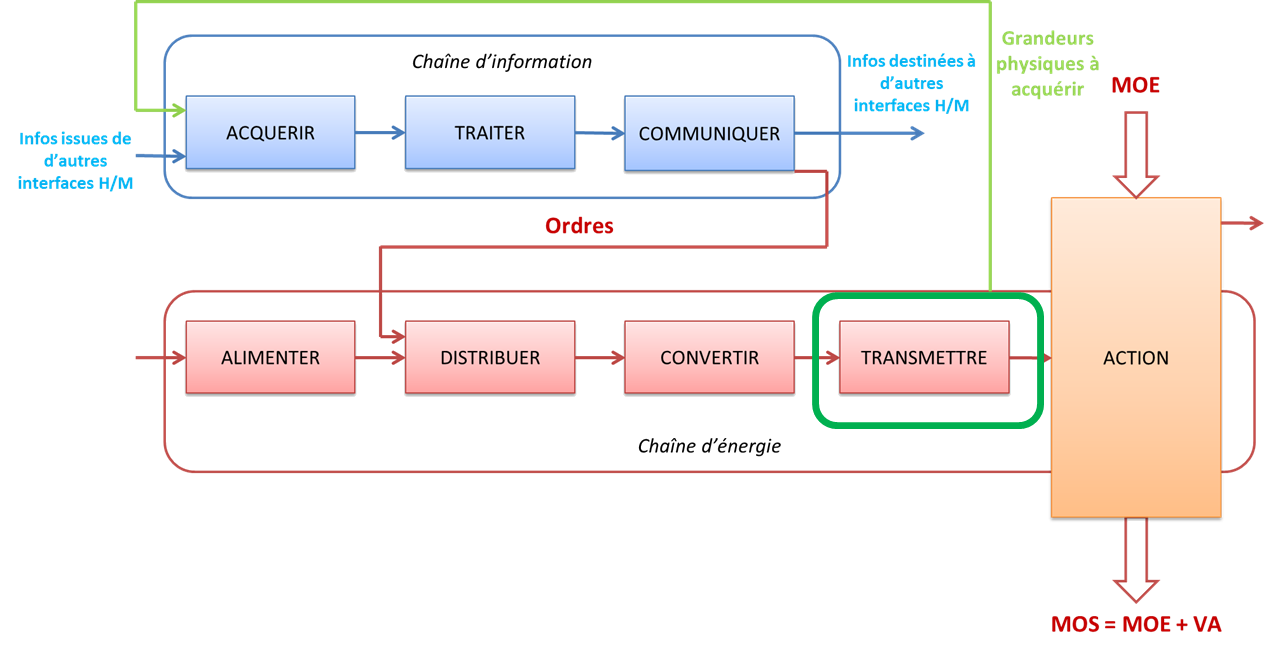
\includegraphics[width=\textwidth]{png/ch_fonc}
\end{center}
\end{minipage}

\begin{center}
\begin{tabular}{ccc}
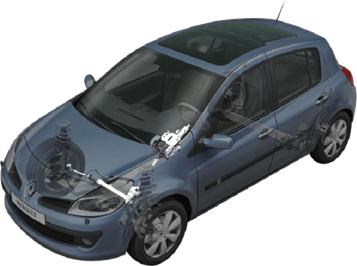
\includegraphics[height=3cm]{png/ex_3} &
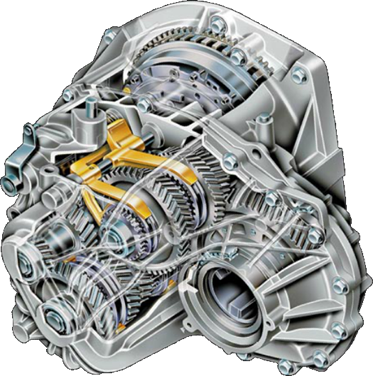
\includegraphics[height=3cm]{png/ex_2} &
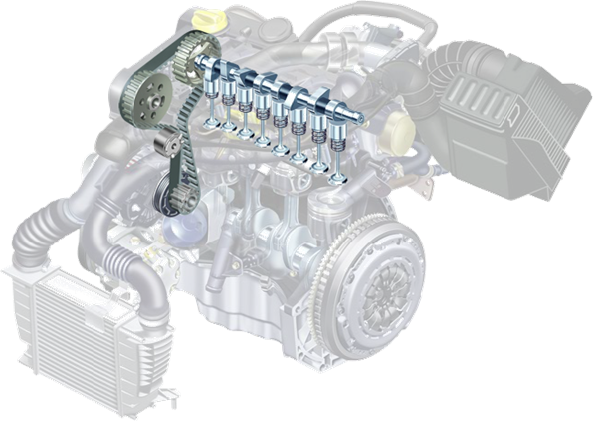
\includegraphics[height=3cm]{png/ex_1} \\
\textit{Système de direction} & \textit{Boîte de vitesse}&\textit{Système de distribution}\\
\end{tabular}
\end{center}

L'étude des différentes parties d'un véhicule permet d'illustrer la richesse des solutions : 
la transformation d'une translation en rotation dans le moteur (système bielle-manivelle), les transmissions par courroie et l'utilisation d'arbre à cames dans le système de distribution, les engrenages et les trains épicycloïdaux dans les boîtes de vitesses et les différentiels...

Le but de ce cours est donc de présenter une liste (non exhaustive) de systèmes de transmission.

\vspace{.2cm}



\begin{prob}
\textsc{Problématique :}
\begin{itemize}
\item Quels sont les systèmes qui permettent de transmettre et de transformer les mouvements ?
\item Comment peut-on modéliser ces systèmes ?
\end{itemize}
\end{prob}

\begin{savoir}
\textsc{Savoirs :}
\begin{itemize}
\item Les transmetteur de puissance mécanique et les effecteurs pour les arbres et accouplements, mécanismes plans à barres, mécanisme vis écrou, réducteurs et multiplicateurs
\end{itemize}
\end{savoir}

\setlength{\parskip}{0ex plus 0.2ex minus 0ex}
 \renewcommand{\contentsname}{}
 \renewcommand{\baselinestretch}{1}

\tableofcontents

 \renewcommand{\baselinestretch}{1.2}
\setlength{\parskip}{2ex plus 0.5ex minus 0.2ex}

% \vspace{1cm}
\textit{Ce document est en évolution permanente. Merci de signaler toutes
erreurs ou coquilles.}


\section{Transmission du mouvement sans modification de la vitesse}
Accouplements




\section{Transmission du mouvement avec modification de la vitesse}

\subsection{Réduction par engrenages}	

\subsubsection{Géométrie des engrenages}

\subsubsection{Train d'engrenages}

\subsection{Trains épicycloïdaux}

\subsection{Réduction par chaîne}
\subsection{Réduction par roue de friction}
\subsection{Variateurs}
 \subsubsection{Variateurs à courroie}
 \subsubsection{Variateurs à friction}
\subsection{Transmission par roue libre}
\section{Transformation du mouvement}
\subsection{Pignon -- Crémaillère}
\subsection{Systèmes bielles manivelles}
\subsection{Systèmes à excentriques}
\subsection{Systèmes à cames}
\subsection{Systèmes à croix malte}
\subsection{Vis - écrou}


\newpage
\subsection{Joint de cardan}
\subsubsection{Description}

\begin{center}
\hfill
\begin{minipage}[c]{.21\linewidth}
\begin{center}
%\includegraphics[width=.9\textwidth]{png/}
\textit{Cas d'utilisation}
\end{center}
\end{minipage} \hfill
\begin{minipage}[c]{.21\linewidth}
\begin{center}
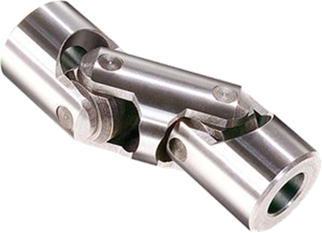
\includegraphics[width=.9\textwidth]{png/cardan2}
\textit{Composant mécanique\cite{cardan2}}
\end{center}
\end{minipage} \hfill
\begin{minipage}[c]{.21\linewidth}
\begin{center}
%\includegraphics[width=.9\textwidth]{png/}
\textit{Modèle CAO}
\end{center} 
\end{minipage}\hfill
\begin{minipage}[c]{.21\linewidth}
\begin{center}
%\includegraphics[width=.9\textwidth]{png/}
\textit{Modèle cinématique}
\end{center} 
\end{minipage}\hfill
\end{center}

Le joint de cardan est utilisé pour transmettre une vitesse de rotation entre deux arbres non coaxiaux (un débattement angulaire est possible entre les deux axes). L'utilisation d'un cardan simple n'est pas homocinétique. Cela signifie que la vitesse de l'arbre moteur et de l'arbre récepteur ne sont pas identiques. Utiliser deux joints de cardan en parallèle permet d'avoir un accouplement homocinétique.



\textbf{Vidéos :}
\begin{itemize}
\item \url{http://www2c.ac-lille.fr/eiffel/cpge/animation25.html}
\end{itemize}

\subsubsection{Modélisation cinématique}
\subsubsection{Modélisation statique}
\subsubsection{Conception}
\subsubsection{Remarques}
\subsubsection{Utilisation}
\begin{itemize}
\item
\end{itemize}

\newpage

\subsection{Joint tripode et joint rzeppa}
\subsubsection{Description}

\begin{center}
\hfill
\begin{minipage}[c]{.21\linewidth}
\begin{center}
%\includegraphics[width=.9\textwidth]{png/}
\textit{Cas d'utilisation}
\end{center}
\end{minipage} \hfill
\begin{minipage}[c]{.21\linewidth}
\begin{center}
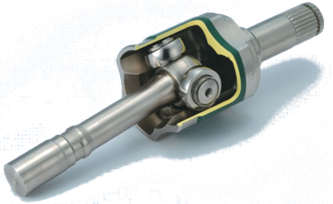
\includegraphics[width=.9\textwidth]{png/tripode2}
\textit{Composant mécanique \cite{tripode2}}
\end{center}
\end{minipage} \hfill
\begin{minipage}[c]{.21\linewidth}
\begin{center}
%\includegraphics[width=.9\textwidth]{png/}
\textit{Modèle CAO}
\end{center} 
\end{minipage}\hfill
\begin{minipage}[c]{.21\linewidth}
\begin{center}
%\includegraphics[width=.9\textwidth]{png/}
\textit{Modèle cinématique}
\end{center} 
\end{minipage}\hfill
\end{center}


\textbf{Vidéos :}
\begin{itemize}
\item
\end{itemize}

\subsubsection{Modélisation cinématique}
\subsubsection{Modélisation statique}
\subsubsection{Conception}
\subsubsection{Remarques}
\subsubsection{Utilisation}
\begin{itemize}
\item
\end{itemize}

\newpage

\subsection{Joint de Oldham}
\subsubsection{Description}

\begin{center}
\hfill
\begin{minipage}[c]{.21\linewidth}
\begin{center}
%\includegraphics[width=.9\textwidth]{png/}
\textit{Cas d'utilisation}
\end{center}
\end{minipage} \hfill
\begin{minipage}[c]{.21\linewidth}
\begin{center}
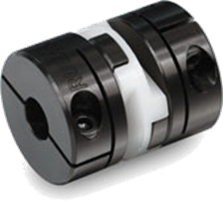
\includegraphics[width=.9\textwidth]{png/oldham2}
\textit{Composant mécanique}
\end{center}
\end{minipage} \hfill
\begin{minipage}[c]{.21\linewidth}
\begin{center}
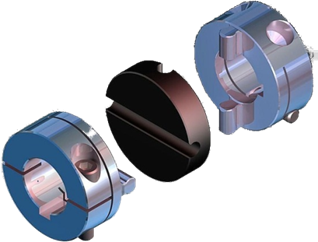
\includegraphics[width=.9\textwidth]{png/oldham3}
\textit{Modèle CAO \cite{oldham3}}
\end{center} 
\end{minipage}\hfill
\begin{minipage}[c]{.21\linewidth}
\begin{center}
%\includegraphics[width=.9\textwidth]{png/}
\textit{Modèle cinématique}
\end{center} 
\end{minipage}\hfill
\end{center}


\textbf{Vidéos :}
\begin{itemize}
\item
\end{itemize}

\subsubsection{Modélisation cinématique}
\subsubsection{Modélisation statique}
\subsubsection{Conception}
\subsubsection{Remarques}
\subsubsection{Utilisation}
\begin{itemize}
\item
\end{itemize}
\newpage

\subsection{Roue libre}
\subsubsection{Description}

\begin{center}
\hfill
\begin{minipage}[c]{.21\linewidth}
\begin{center}
%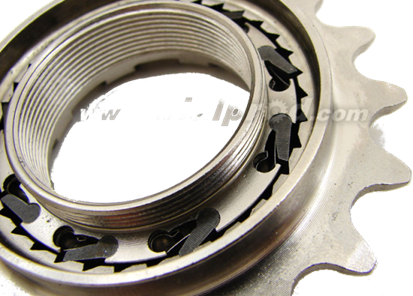
\includegraphics[width=.9\textwidth]{png/roue_1}
\textit{Cas d'utilisation}
\end{center}
\end{minipage} \hfill
\begin{minipage}[c]{.21\linewidth}
\begin{center}
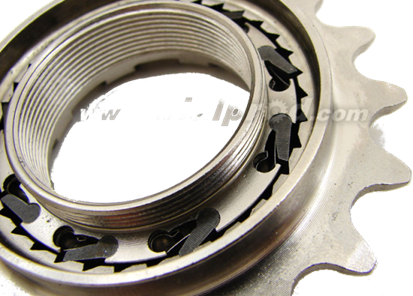
\includegraphics[width=.9\textwidth]{png/roue_1}
\textit{Composant mécanique \cite{roue1}}
\end{center}
\end{minipage} \hfill
\begin{minipage}[c]{.21\linewidth}
\begin{center}
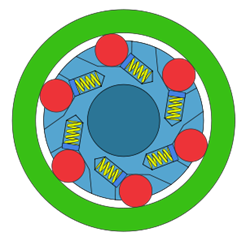
\includegraphics[width=.9\textwidth]{png/roue_2}
\textit{Représentation graphique \cite{roue2}}
\end{center} 
\end{minipage}\hfill
\begin{minipage}[c]{.21\linewidth}
\begin{center}
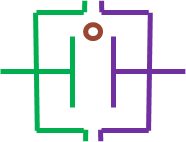
\includegraphics[width=.9\textwidth]{png/roue_4}
\textit{Modèle cinématique}
\end{center} 
\end{minipage}\hfill
\end{center}


\textbf{Vidéos :}
\begin{itemize}
\item
\end{itemize}

\subsubsection{Modélisation cinématique}
\subsubsection{Modélisation statique}
\subsubsection{Conception}
\subsubsection{Remarques}
\subsubsection{Utilisation}
\begin{itemize}
\item
\end{itemize}
\newpage

\subsection{Embrayages}
\subsubsection{Description}

\begin{center}
\hfill
\begin{minipage}[c]{.21\linewidth}
\begin{center}
%\includegraphics[width=.9\textwidth]{png/}
\textit{Cas d'utilisation}
\end{center}
\end{minipage} \hfill
\begin{minipage}[c]{.21\linewidth}
\begin{center}
%\includegraphics[width=.9\textwidth]{png/}
\textit{Composant mécanique}
\end{center}
\end{minipage} \hfill
\begin{minipage}[c]{.21\linewidth}
\begin{center}
%\includegraphics[width=.9\textwidth]{png/}
\textit{Modèle CAO}
\end{center} 
\end{minipage}\hfill
\begin{minipage}[c]{.21\linewidth}
\begin{center}
%\includegraphics[width=.9\textwidth]{png/}
\textit{Modèle cinématique}
\end{center} 
\end{minipage}\hfill
\end{center}


\textbf{Vidéos :}
\begin{itemize}
\item
\end{itemize}

\subsubsection{Modélisation cinématique}
\subsubsection{Modélisation statique}
\subsubsection{Conception}
\subsubsection{Remarques}
\subsubsection{Utilisation}
\begin{itemize}
\item
\end{itemize}
\newpage

\subsection{Train d'engrenage simple}
\subsubsection{Description}

\begin{center}
\hfill
\begin{minipage}[c]{.21\linewidth}
\begin{center}
%\includegraphics[width=.9\textwidth]{png/}
\textit{Cas d'utilisation}
\end{center}
\end{minipage} \hfill
\begin{minipage}[c]{.21\linewidth}
\begin{center}
%\includegraphics[width=.9\textwidth]{png/}
\textit{Composant mécanique}
\end{center}
\end{minipage} \hfill
\begin{minipage}[c]{.21\linewidth}
\begin{center}
%\includegraphics[width=.9\textwidth]{png/}
\textit{Modèle CAO}
\end{center} 
\end{minipage}\hfill
\begin{minipage}[c]{.21\linewidth}
\begin{center}
%\includegraphics[width=.9\textwidth]{png/}
\textit{Modèle cinématique}
\end{center} 
\end{minipage}\hfill
\end{center}


\textbf{Vidéos :}
\begin{itemize}
\item
\end{itemize}

\subsubsection{Modélisation cinématique}
\subsubsection{Modélisation statique}
\subsubsection{Conception}
\subsubsection{Remarques}
\subsubsection{Utilisation}
\begin{itemize}
\item
\end{itemize}
\newpage

\subsection{Train d'engrenage épicycloïdal}
\subsubsection{Description}

\begin{center}
\hfill
\begin{minipage}[c]{.21\linewidth}
\begin{center}
%\includegraphics[width=.9\textwidth]{png/}
\textit{Cas d'utilisation}
\end{center}
\end{minipage} \hfill
\begin{minipage}[c]{.21\linewidth}
\begin{center}
%\includegraphics[width=.9\textwidth]{png/}
\textit{Composant mécanique}
\end{center}
\end{minipage} \hfill
\begin{minipage}[c]{.21\linewidth}
\begin{center}
%\includegraphics[width=.9\textwidth]{png/}
\textit{Modèle CAO}
\end{center} 
\end{minipage}\hfill
\begin{minipage}[c]{.21\linewidth}
\begin{center}
%\includegraphics[width=.9\textwidth]{png/}
\textit{Modèle cinématique}
\end{center} 
\end{minipage}\hfill
\end{center}


\textbf{Vidéos :}
\begin{itemize}
\item
\end{itemize}

\subsubsection{Modélisation cinématique}
\subsubsection{Modélisation statique}
\subsubsection{Conception}
\subsubsection{Remarques}
\subsubsection{Utilisation}
\begin{itemize}
\item
\end{itemize}
\newpage

\subsection{Transmission par chaîne et par courroie}
\subsubsection{Description}

\begin{center}
\hfill
\begin{minipage}[c]{.21\linewidth}
\begin{center}
%\includegraphics[width=.9\textwidth]{png/}
\textit{Cas d'utilisation}
\end{center}
\end{minipage} \hfill
\begin{minipage}[c]{.21\linewidth}
\begin{center}
%\includegraphics[width=.9\textwidth]{png/}
\textit{Composant mécanique}
\end{center}
\end{minipage} \hfill
\begin{minipage}[c]{.21\linewidth}
\begin{center}
%\includegraphics[width=.9\textwidth]{png/}
\textit{Modèle CAO}
\end{center} 
\end{minipage}\hfill
\begin{minipage}[c]{.21\linewidth}
\begin{center}
%\includegraphics[width=.9\textwidth]{png/}
\textit{Modèle cinématique}
\end{center} 
\end{minipage}\hfill
\end{center}


\textbf{Vidéos :}
\begin{itemize}
\item
\end{itemize}

\subsubsection{Modélisation cinématique}
\subsubsection{Modélisation statique}
\subsubsection{Conception}
\subsubsection{Remarques}
\subsubsection{Utilisation}
\begin{itemize}
\item
\end{itemize}
\newpage

\subsection{Transmission par friction}
\subsubsection{Description}

\begin{center}
\hfill
\begin{minipage}[c]{.21\linewidth}
\begin{center}
%\includegraphics[width=.9\textwidth]{png/}
\textit{Cas d'utilisation}
\end{center}
\end{minipage} \hfill
\begin{minipage}[c]{.21\linewidth}
\begin{center}
%\includegraphics[width=.9\textwidth]{png/}
\textit{Composant mécanique}
\end{center}
\end{minipage} \hfill
\begin{minipage}[c]{.21\linewidth}
\begin{center}
%\includegraphics[width=.9\textwidth]{png/}
\textit{Modèle CAO}
\end{center} 
\end{minipage}\hfill
\begin{minipage}[c]{.21\linewidth}
\begin{center}
%\includegraphics[width=.9\textwidth]{png/}
\textit{Modèle cinématique}
\end{center} 
\end{minipage}\hfill
\end{center}


\textbf{Vidéos :}
\begin{itemize}
\item
\end{itemize}

\subsubsection{Modélisation cinématique}
\subsubsection{Modélisation statique}
\subsubsection{Conception}
\subsubsection{Remarques}
\subsubsection{Utilisation}
\begin{itemize}
\item
\end{itemize}
\newpage

\subsection{Pignon -- crémaillère}
\subsubsection{Description}

\begin{center}
\hfill
\begin{minipage}[c]{.21\linewidth}
\begin{center}
%\includegraphics[width=.9\textwidth]{png/}
\textit{Cas d'utilisation}
\end{center}
\end{minipage} \hfill
\begin{minipage}[c]{.21\linewidth}
\begin{center}
%\includegraphics[width=.9\textwidth]{png/}
\textit{Composant mécanique}
\end{center}
\end{minipage} \hfill
\begin{minipage}[c]{.21\linewidth}
\begin{center}
%\includegraphics[width=.9\textwidth]{png/}
\textit{Modèle CAO}
\end{center} 
\end{minipage}\hfill
\begin{minipage}[c]{.21\linewidth}
\begin{center}
%\includegraphics[width=.9\textwidth]{png/}
\textit{Modèle cinématique}
\end{center} 
\end{minipage}\hfill
\end{center}


\textbf{Vidéos :}
\begin{itemize}
\item
\end{itemize}

\subsubsection{Modélisation cinématique}
\subsubsection{Modélisation statique}
\subsubsection{Conception}
\subsubsection{Remarques}
\subsubsection{Utilisation}
\begin{itemize}
\item
\end{itemize}
\newpage

\subsection{Bielle -- manivelle}
\subsubsection{Description}

\begin{center}
\hfill
\begin{minipage}[c]{.21\linewidth}
\begin{center}
%\includegraphics[width=.9\textwidth]{png/}
\textit{Cas d'utilisation}
\end{center}
\end{minipage} \hfill
\begin{minipage}[c]{.21\linewidth}
\begin{center}
%\includegraphics[width=.9\textwidth]{png/}
\textit{Composant mécanique}
\end{center}
\end{minipage} \hfill
\begin{minipage}[c]{.21\linewidth}
\begin{center}
%\includegraphics[width=.9\textwidth]{png/}
\textit{Modèle CAO}
\end{center} 
\end{minipage}\hfill
\begin{minipage}[c]{.21\linewidth}
\begin{center}
%\includegraphics[width=.9\textwidth]{png/}
\textit{Modèle cinématique}
\end{center} 
\end{minipage}\hfill
\end{center}


\textbf{Vidéos :}
\begin{itemize}
\item
\end{itemize}

\subsubsection{Modélisation cinématique}
\subsubsection{Modélisation statique}
\subsubsection{Conception}
\subsubsection{Remarques}
\subsubsection{Utilisation}
\begin{itemize}
\item
\end{itemize}
\newpage

\subsection{Cames}
\subsubsection{Description}

\begin{center}
\hfill
\begin{minipage}[c]{.21\linewidth}
\begin{center}
%\includegraphics[width=.9\textwidth]{png/}
\textit{Cas d'utilisation}
\end{center}
\end{minipage} \hfill
\begin{minipage}[c]{.21\linewidth}
\begin{center}
%\includegraphics[width=.9\textwidth]{png/}
\textit{Composant mécanique}
\end{center}
\end{minipage} \hfill
\begin{minipage}[c]{.21\linewidth}
\begin{center}
%\includegraphics[width=.9\textwidth]{png/}
\textit{Modèle CAO}
\end{center} 
\end{minipage}\hfill
\begin{minipage}[c]{.21\linewidth}
\begin{center}
%\includegraphics[width=.9\textwidth]{png/}
\textit{Modèle cinématique}
\end{center} 
\end{minipage}\hfill
\end{center}


\textbf{Vidéos :}
\begin{itemize}
\item
\end{itemize}

\subsubsection{Modélisation cinématique}
\subsubsection{Modélisation statique}
\subsubsection{Conception}
\subsubsection{Remarques}
\subsubsection{Utilisation}
\begin{itemize}
\item
\end{itemize}
\newpage

\subsection{Excentriques}
\subsubsection{Description}

\begin{center}
\hfill
\begin{minipage}[c]{.21\linewidth}
\begin{center}
%\includegraphics[width=.9\textwidth]{png/}
\textit{Cas d'utilisation}
\end{center}
\end{minipage} \hfill
\begin{minipage}[c]{.21\linewidth}
\begin{center}
%\includegraphics[width=.9\textwidth]{png/}
\textit{Composant mécanique}
\end{center}
\end{minipage} \hfill
\begin{minipage}[c]{.21\linewidth}
\begin{center}
%\includegraphics[width=.9\textwidth]{png/}
\textit{Modèle CAO}
\end{center} 
\end{minipage}\hfill
\begin{minipage}[c]{.21\linewidth}
\begin{center}
%\includegraphics[width=.9\textwidth]{png/}
\textit{Modèle cinématique}
\end{center} 
\end{minipage}\hfill
\end{center}


\textbf{Vidéos :}
\begin{itemize}
\item
\end{itemize}

\subsubsection{Modélisation cinématique}
\subsubsection{Modélisation statique}
\subsubsection{Conception}
\subsubsection{Remarques}
\subsubsection{Utilisation}
\begin{itemize}
\item
\end{itemize}
\newpage

\subsection{Croix de Malte}
\subsubsection{Description}

\begin{center}
\hfill
\begin{minipage}[c]{.21\linewidth}
\begin{center}
%\includegraphics[width=.9\textwidth]{png/}
\textit{Cas d'utilisation}
\end{center}
\end{minipage} \hfill
\begin{minipage}[c]{.21\linewidth}
\begin{center}
%\includegraphics[width=.9\textwidth]{png/}
\textit{Composant mécanique}
\end{center}
\end{minipage} \hfill
\begin{minipage}[c]{.21\linewidth}
\begin{center}
%\includegraphics[width=.9\textwidth]{png/}
\textit{Modèle CAO}
\end{center} 
\end{minipage}\hfill
\begin{minipage}[c]{.21\linewidth}
\begin{center}
%\includegraphics[width=.9\textwidth]{png/}
\textit{Modèle cinématique}
\end{center} 
\end{minipage}\hfill
\end{center}


\textbf{Vidéos :}
\begin{itemize}
\item
\end{itemize}

\subsubsection{Modélisation cinématique}
\subsubsection{Modélisation statique}
\subsubsection{Conception}
\subsubsection{Remarques}
\subsubsection{Utilisation}
\begin{itemize}
\item
\end{itemize}

\newpage

\subsection{Vis -- écrou}
\subsubsection{Description}

\begin{center}
\hfill
\begin{minipage}[c]{.21\linewidth}
\begin{center}
%\includegraphics[width=.9\textwidth]{png/}
\textit{Cas d'utilisation}
\end{center}
\end{minipage} \hfill
\begin{minipage}[c]{.21\linewidth}
\begin{center}
%\includegraphics[width=.9\textwidth]{png/}
\textit{Composant mécanique}
\end{center}
\end{minipage} \hfill
\begin{minipage}[c]{.21\linewidth}
\begin{center}
%\includegraphics[width=.9\textwidth]{png/}
\textit{Modèle CAO}
\end{center} 
\end{minipage}\hfill
\begin{minipage}[c]{.21\linewidth}
\begin{center}
%\includegraphics[width=.9\textwidth]{png/}
\textit{Modèle cinématique}
\end{center} 
\end{minipage}\hfill
\end{center}


\textbf{Vidéos :}
\begin{itemize}
\item
\end{itemize}

\subsubsection{Modélisation cinématique}
\subsubsection{Modélisation statique}
\subsubsection{Conception}
\subsubsection{Remarques}
\subsubsection{Utilisation}
\begin{itemize}
\item
\end{itemize}

\begin{itemize}
\item
\end{itemize}
\newpage

\subsection{Roue et vis sans fin}
\subsubsection{Description}

\begin{center}
\hfill
\begin{minipage}[c]{.21\linewidth}
\begin{center}
%\includegraphics[width=.9\textwidth]{png/}
\textit{Cas d'utilisation}
\end{center}
\end{minipage} \hfill
\begin{minipage}[c]{.21\linewidth}
\begin{center}
%\includegraphics[width=.9\textwidth]{png/}
\textit{Composant mécanique}
\end{center}
\end{minipage} \hfill
\begin{minipage}[c]{.21\linewidth}
\begin{center}
%\includegraphics[width=.9\textwidth]{png/}
\textit{Modèle CAO}
\end{center} 
\end{minipage}\hfill
\begin{minipage}[c]{.21\linewidth}
\begin{center}
%\includegraphics[width=.9\textwidth]{png/}
\textit{Modèle cinématique}
\end{center} 
\end{minipage}\hfill
\end{center}


\textbf{Vidéos :}
\begin{itemize}
\item 
\end{itemize}

\subsubsection{Modélisation cinématique}
\subsubsection{Modélisation statique}
\subsubsection{Conception}
\subsubsection{Remarques}
\subsubsection{Utilisation}
\begin{itemize}
\item
\end{itemize}
\begin{itemize}
\item
\end{itemize}

\begin{thebibliography}{2}
\bibitem{cardan2}{\url{http://img.directindustry.fr/images_di/photo-m2/cardans-doubles-379839.jpg}}
\bibitem{tripode2}{\url{http://2.bp.blogspot.com/-EFFAq8t0O7U/TfUzsiwoG5I/AAAAAAAAAFE/TvOfMzMTO3w/s1600/tripodjoint.jpg}}
\bibitem{oldham3}{\url{http://img.directindustry.fr/images_di/photo-g/accouplement-flexible-accouplement-oldham-422127.jpg}}

\bibitem{roue1}{\url{http://www.trialprod.com/fr/}}
\bibitem{roue2}{\url{http://fr.wikipedia.org/wiki/Fichier:Roue_libre2.svg}}

\end{thebibliography}

\end{document}